\section{Theoretical and Conceptual Framework}
Figure \ref{tcf} shows the Theoretical and Conceptual Framework of this study which outlines the methods, strategies, and algorithms this study plans to adopt from previous research. It also shows how all these connect to this study's objectives. The framework is divided into three (3) sections:

    \begin{enumerate}
        \item The \textit{Requirements Definition} focuses on introducing and elucidating the concepts upon which this study is built. These concepts include workflows and workflow dimensions, RDLT and Petri Net definitions, and notations, as well as RDLT and Petri Net soundness.
        \item The \textit{Requirements Specification} aims to identify components and concepts in RDLT that are used in the mapping presented in \cite{sulla-malinao} as well as the gaps in that proposed mapping. Also, extensions/variants of Petri Net that can be used in improving the full mapping of RDLT to PN are identified.
        \item The \textit{Implementation} section aims to improve the full mapping of RDLT to Petri Net with consideration of the RBS using identified components or extensions/variants of PN and some concepts used in the previous mapping presented in \cite{sulla-malinao}. The implications of this mapping with respect to Petri net soundness will also be reported.
    \end{enumerate}

    \begin{figure}[p]
        \centering
        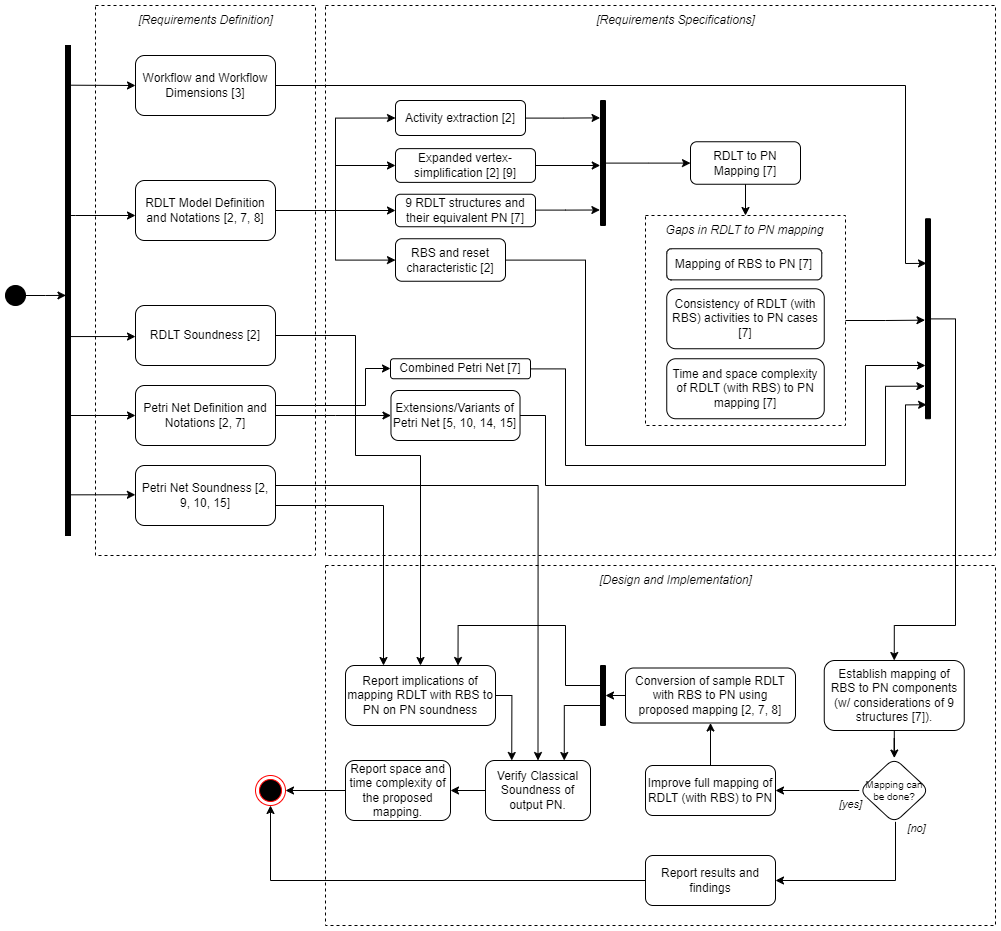
\includegraphics[scale=0.5]{figures/TCF_V5.png}
        \caption{The Theoretical and Conceptual Framework.}
        \label{tcf}
    \end{figure} \par